\documentclass[tikz]{standalone}

\begin{document}
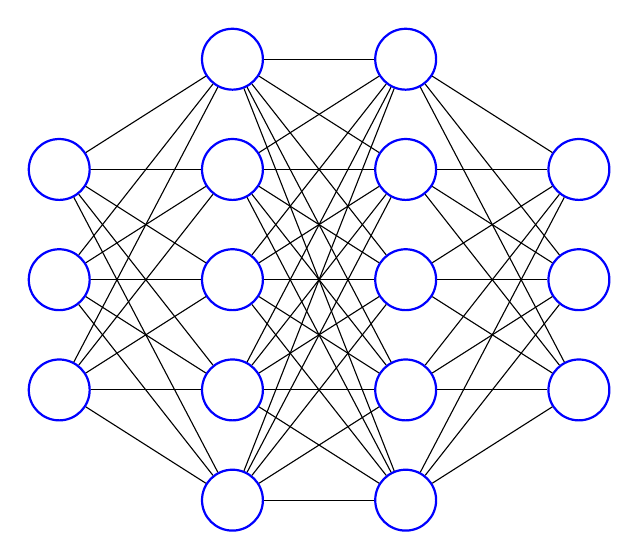
\begin{tikzpicture}[x=2.2cm,y=1.4cm,
    mynode/.style = {thick, draw=blue, circle, minimum size=22}
  ]
  \foreach \N [count=\lay,remember={\N as \Nprev (initially 0);}]
  in {3,5,5,3}{ % loop over layers
      \foreach \i [evaluate={\y=\N/2-\i; \x=\lay; \prev=int(\lay-1);}]
      in {1,...,\N}{ % loop over nodes
          \node[mynode] (N\lay-\i) at (\x,\y) {};
          \ifnum\Nprev>0 % connect to previous layer
            \foreach \j in {1,...,\Nprev}{ % loop over nodes in previous layer
                \draw[thin] (N\prev-\j) -> (N\lay-\i);
              }
          \fi
        }
    }

\end{tikzpicture}
\end{document}
